\documentclass[11pt, oneside]{article}   	% use "amsart" instead of "article" for AMSLaTeX format
\usepackage{geometry}                		% See geometry.pdf to learn the layout options. There are lots.
\geometry{letterpaper}                   		% ... or a4paper or a5paper or ... 
%\geometry{landscape}                		% Activate for rotated page geometry
%\usepackage[parfill]{parskip}    		% Activate to begin paragraphs with an empty line rather than an indent
\usepackage{graphicx}				% Use pdf, png, jpg, or eps§ with pdflatex; use eps in DVI mode
								% TeX will automatically convert eps --> pdf in pdflatex	
\usepackage{amssymb}
\usepackage[tbtags]{amsmath}
\usepackage{tikz}
\usepackage{pgfplots}
\pgfplotsset{width=6cm,compat=1.9}
\usepackage[toc,page]{appendix}
\usepackage{graphicx}
\graphicspath{ {images/} }

\title{Fast multipole methods for axisymmetric geometries}
\author{Victor Churchill\\New York University}
\date{May 13, 2016}

\begin{document}
\maketitle

\begin{abstract}
Fast multipole methods (FMMs) are one of the main numerical methods used in the solution of integral equations arising from the boundary-value PDEs of classical mathematical physics. When the boundary to be discretized possesses rotational symmetry, however, Fast Fourier Transforms can be used to decompose the surface integral equation into a series of integral equations along curves. The kernels of these integral equations are the Fourier modes of the original three-dimensional Green's function.

In this work, we extend the idea of interpolation-based fast multipole methods to kernels which are \textit{not} translation invariant, in particular, modal Green's functions. Building on the previous work of Fong and Darve, 2009, we show that Black Box FMMs can be constructed for modal Green's functions which can take advantage of efficient BLAS3 linear algebra routines, effectively vectorizing the calculation across all rotational modes.
\end{abstract}

\section{Introduction}
This project examines the problem of constructing of a fast multipole method (FMM) algorithm for density distributions on axisymmetric surfaces of revolution. Using the symmetry of the surface, Fourier methods can be used to represent free-space three-dimensional Green's functions in terms of their angular Fourier modes. These kernels are known as modal Green's functions. We will refer to the resulting numerical scheme as the \textit{modal FMM} (mFMM).

We will work in three-dimensional cylindrical coordinates $(r,\theta,z)$ such that a point in Cartesian coordinates $(x,y,z)$ is represented by:

\begin{align*}
x &= r\cos\theta\\
y &= r\sin\theta\\
z &= z
\end{align*}

An axisymmetric, or rotationally symmetric, surface $\Gamma$ is obtained by rotating a two-dimensional curve $\gamma$ about the $z$ axis. The curve $\gamma$ is called the generating curve, as in Figure \ref{fig:1}. In particular, $\Gamma=\gamma\times\mathbb{T}$ where $\mathbb{T}$ is the one-dimensional torus (circle) parametrized by $\theta\in(-\pi,\pi]$.

\begin{figure}[h]
\caption{An axisymmetric bowl-shaped surface $\Gamma$ and its generating curve $\gamma$.}
\label{fig:1}
\centering
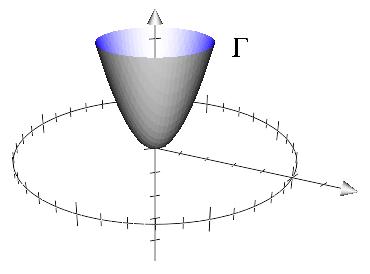
\includegraphics[scale=0.5]{./images/bowl3}
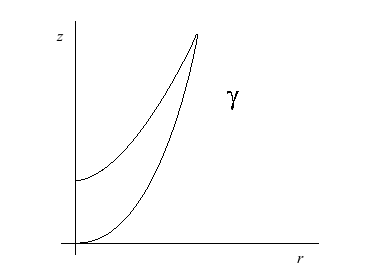
\includegraphics[scale=0.5]{./images/bowl}
\end{figure}

Integral equations are equations using integral operators defines on curves or surfaces. For example, consider the integral equation
\begin{align}
f(\mathbf{x}) &= \int_\Gamma K(\mathbf{x},\mathbf{y})\sigma(\mathbf{y})d\mathbf{y} &\mathbf{x},\mathbf{y}\in\Gamma
\end{align}
where $f$ is a potential, $K$ is the kernel, and $\sigma$ is a continuous density distribution. Boundary integral equations of this form can be solved for $f$ by using a discretization scheme.
\begin{align}
f(\mathbf{x}) = \sum_{j=1}^N K(\mathbf{x},\mathbf{y}_j)\sigma_j &&\mathbf{x},\mathbf{y}_j\in\Gamma
\end{align}
The discretization from the integral equation to a discrete sum over a finite number of points requires a numerical quadrature rule for approximating the integral which specifies the location and spacing of, as well as the weights at, the discretization points, as well as interpolation functions (polynomials).

Integral equations over surfaces and curves with corners or geometric singularities are more difficult to discretize than smooth curves and surfaces. For example, a circular generating curve like in Figure \ref{fig:2} is easy to discretize with a relatively low number of equally-spaced points (simple numerical quadrature). For a rectangular generating curve like in Figure \ref{fig:3}, however, we need more discretization points in the corners due to this source density clumping. Similarly, for a bowl-shaped surface as in Figure \ref{fig:1}, we would need a lot of discretization points near the vertex of the generating curve. The need for a modal FMM arises from this difficulty of discretizing axisymmetric boundary-value integral equations with corners or geometric singularities such that source densities clump together and require a large number of discretization points to be well-represented.
\begin{figure}[h]
\caption{An axisymmetric torus $\Gamma$ and its circular generating curve $\gamma$.}
\label{fig:2}
\centering
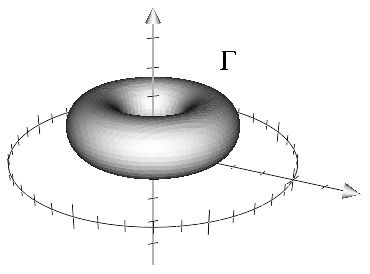
\includegraphics[scale=0.5]{./images/torus}
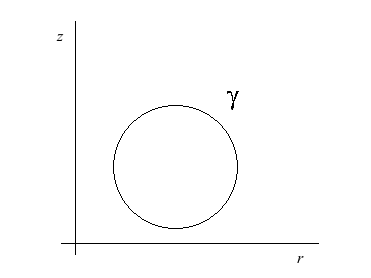
\includegraphics[scale=0.5]{./images/circle}
\end{figure}
\begin{figure}[h]
\caption{An axisymmetric pipe surface $\Gamma$ and its rectangular generating curve $\gamma$.}
\label{fig:3}
\centering
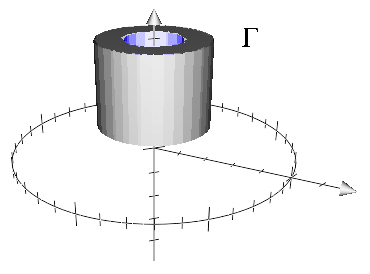
\includegraphics[scale=0.5]{./images/pipe2}
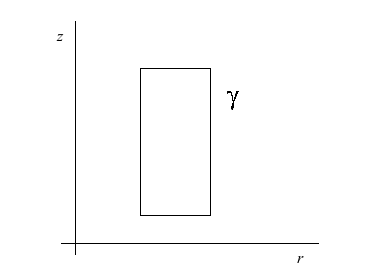
\includegraphics[scale=0.5]{./images/rect}
\end{figure}

Integral equations on axisymmetric surfaces have many applications. The problem of electromagnetic scattering by a surface of revolution, for example, has radar, geophysical exploration, and acoustics applications. Fast direct solvers, like the one proposed in \cite{HMY}, rely on FMM-type rank observations for axisymmetric density distributions to help solve problems arising in these fields.

The remaining organization of this paper is as follows: $\S2$ states the problem in detail. $\S3$ gives the motivation for using and the derivation of the Fourier representation of a Green's function. $\S4$ gives an overview of fast multipole methods and discusses why some existing techniques are not optimal for geometrically-challenging axisymmetric distributions. $\S5$ details the black-box Chebyshev interpolation-based FMM as a basis for the modal FMM. Lastly, $\S6$ describes future work to construct, implement and test a full modal FMM algorithm.

\section{Statement of problem}
Motivate using layer potential instead of N-body problem, otherwise points need to be equidistantly spaced in $\theta$.

Consider the integral equation
\begin{align}
f(\mathbf{x}_i) &= \int_\Gamma K(\mathbf{x}_i,\mathbf{y})\sigma(\mathbf{y})d\mathbf{y} &\mathbf{x}_i,\mathbf{y}\in\Gamma
\end{align}

where $K$ is a layer potential kernel, and $\sigma$ is a given continuous density or charge distribution. We want to compute the potential $f$  at targets $\mathbf{x}_i$ due to sources $\mathbf{y}$.

Consider $N$ source points $\mathbf{y}_j=(r'_j,\theta'_j,z'_j)$ distributed on an axisymmetric surface $\Gamma$, with each assigned a charge $\sigma_j$. In practice, the same set of points act as both sources and targets. The potential is represented by the sum
\begin{align}
f(\mathbf{x}_i) = \sum_{j=1}^N K(\mathbf{x}_i,\mathbf{y}_j)\sigma_j
\end{align}
where $K(\mathbf{x},\mathbf{y})$ is a kernel, typically the Green's function of the partial differential equation that describes the potential between two points in the domain. In particular, we are interested in the free-space (no boundary conditions) Green's function for Laplace's equation, $\Delta u = 0$:
\begin{align}
K(\mathbf{x},\mathbf{y}) = \frac{1}{4\pi |\mathbf{x}-\mathbf{y}|}
\end{align}

The goal is to construct a fast summation method for this integral equation that takes advantage of the rotational symmetry of $\Gamma$ using a discretization scheme and numerical quadrature rule that accounts for geometric structures with corners or geometric singularities.

\section{Modal Green's Function}

The crucial technique to construct a fast method for an axisymmetric density distribution is to reduce the problem in three dimensions to a series of problems in two dimensions using Fourier analysis. In $\S3.1$, we show the derivation of this Fourier representation for an arbitrary kernel, then for the Green's function of Laplace's equation. This strategy is grounded in the fact that it is easier to solve boundary integral equations defined on curves in $\mathbb{R}^2$ than those defined on surfaces in $\mathbb{R}^3$.

We are able to reduce the problem in this way because the rotationally symmetric nature of $\Gamma$ yields $K(\mathbf{x},\mathbf{y})$ symmetric along the $\theta$-axis such that the kernel is a function of the difference $\theta-\theta'$:
\begin{align*}
K(\mathbf{x},\mathbf{y})=K(\theta-\theta',r,z,r',z')
\end{align*}
We call such a kernel rotationally invariant.

Now recall that if for two any points $\mathbf{x}$ and $\mathbf{y}$ in the computational domain a kernel can be written
\begin{align*}
K(\mathbf{x},\mathbf{y}) = K(|\mathbf{x}-\mathbf{y}|)
\end{align*}
then it is called translation invariant. Every translation invariant kernel is also rotationally invariant. Notice that the Green's function for Laplace's equation is translation invariant. Not all kernels are translation invariant, however, and the fact that what we'll define in $\S3.1$ as the modal Green's function is not translation invariant is crucial to the difficulty of creating a modal FMM.

\subsection{Fourier representation of 3D integral equations}
This derivation closely follows \cite{YYM}. Consider the Fredholm integral equation of the first kind defined on $\Gamma$:
\begin{align}
f(\mathbf{x}) &= \int_\Gamma K(\mathbf{x},\mathbf{y})\sigma(\mathbf{y})d\mathbf{y} &\mathbf{x},\mathbf{y}\in\Gamma
\end{align}
This is a 3D integral equation, which we can view as a continuous version of equation $(1)$.

We can represent $(3)$ as a sequence of 2D integral equations defined on the generating curve $\gamma$ by performing Fourier transformations on $f$, $\sigma$, and $K$. If $f_m$, $\sigma_m$, and $k_m$ are the Fourier modes of $f$, $\sigma$, and $K$, respectively, then we have
\begin{align*}
f_m(r,z)&=\int_\mathbb{T}\frac{e^{-im\theta}}{\sqrt{2\pi}}f(r,z,\theta)d\theta&f(\mathbf{x})&=\sum_{m\in\mathbb{Z}}\frac{e^{im\theta}}{\sqrt{2\pi}}f_m(r,z)\\
\sigma_m(r,z)&=\int_\mathbb{T}\frac{e^{-im\theta}}{\sqrt{2\pi}}\sigma(r,z,\theta)d\theta&\sigma(\mathbf{x})&=\sum_{m\in\mathbb{Z}}\frac{e^{im\theta}}{\sqrt{2\pi}}\sigma_m(r,z)\\
k_m(r,z,r',z')&=\int_\mathbb{T}\frac{e^{-im\theta}}{\sqrt{2\pi}}K(r,z,r',z',\theta)d\theta&K(\mathbf{x},\mathbf{y})&=\sum_{m\in\mathbb{Z}}\frac{e^{im(\theta-\theta')}}{\sqrt{2\pi}}k_m(r,z,r',z')
\end{align*}
such that
\begin{align}
\sqrt{2\pi}\int_\gamma k_m(r,z,r',z')\sigma_m(r',z')r'dl(r',z')&=f_m(r,z) &(r,z),(r',z')\in\gamma
\end{align}
for each $m\in\mathbb{Z}$.

In practice, we choose a truncation parameter, $M\in\mathbb{N}$, such that $f$ is well-represented by its lowest $2M+1$ Fourier modes
\begin{align}
||f-\sum\limits_{m=-M}^{M}\frac{e^{im\theta}}{\sqrt{2\pi}}f_m||\le\epsilon
\end{align}
and only utilize the lowest $2M+1$ Fourier modes for each of the functions $f$, $\sigma$, and $K$.

We are using the Green's function of a PDE as our kernel, so $k_m$ is called the modal Green's function. We should note that for now we are only considering the Green's function for Laplace's equation because its Fourier modes can be solved for analytically. For many other kernels, it is not possible to find the same type of explicit formula, and we would need to approximate the modes using a discretization as in \cite{YYM}. So for the Green's function for Laplace's equation we have
\begin{align}
\frac{1}{4\pi |\mathbf{x}-\mathbf{y}|} &=\frac{1}{4\pi\sqrt{r^2+r'^2-2rr'\cos{(\theta-\theta')}+(z-z')^2}}\\
&= \sum_{m\in\mathbb{Z}} \frac{e^{im(\theta-\theta')}}{\sqrt{2\pi}} s_m(r,z,r',z')
\end{align}
where the modal Green's function is
\begin{align}
s_m(r,z,r',z')=\frac{1}{\sqrt{8\pi^3 rr'}}\mathbf{Q}_{m-\frac{1}{2}}\bigg(\frac{r^2+(r')^2+(z-z')^2}{2rr'}\bigg)
\end{align}
with $Q_{m-\frac{1}{2}}$ the half-integer order Legendre function of the second kind. Notice that while $K$ was translation invariant, $s_m$ is not. This has implications which we discuss later.

Now rather than constructing a fast summation for a density distribution on $\Gamma$ using $K(\mathbf{x},\mathbf{y})$, we can construct a series of fast summations for a density distribution on $\gamma$ using $s_m(r,z,r',z')$.

In the next section, we give an overview of the FMM, and discuss how several well-known fast methods approach the problem of axisymmetric density distributions.

\section{Fast multipole methods}
Fast multipole methods are a class of algorithms that were developed to compute $N$-body sums in $\mathcal{O}(N)$ time. FMMs are widely used in combination with iterative solvers to find the solutions of integral equations. Equation $(1)$ shows the naive computation of such a potential. We can view this as a matrix-vector multiplication. In general, FMMs reduce the computational complexity of this matrix-vector multiplication from $\mathcal{O}(N^2)$ to $\mathcal{O}(N)$ or $\mathcal{O}(N\log N)$ for a given error level $\epsilon$. FMMs are fast approximation algorithms, with higher accuracy costing higher computational complexity. There are two fundamental categories of FMMs that differ in the way that they efficiently represent source densities: analysis-based algorithms that use analytic multipole and local expansions, and kernel-independent methods that use equivalent densities or weights.

In the analysis-based FMM, the potential induced by source densities at a far away target is represented using a multipole expansion, while the potential induced by the far away sources is encoded in a local expansion. In kernel-independent methods, the potential induced by source densities at a far away target is represented using an upward equivalent density, while the potential induced by far away sources is encoded using a downward equivalent density. Each of these interactions is low-rank, and can be approximated using low-degree interpolation or special function expansions. The basic idea is that for well-separated points, the naively-computed potential between sources and targets is the same as the potential due to the efficient density representation. The target points can't tell the difference between the actual source densities and the density representation, so we can take advantage of the fact that it's less computationally expensive to use these representations.

\subsection{Hierarchical tree structure}
Before we discuss these two types of FMMs further, we need to define the tree structure of the computational domain which allows us to specify what we mean by "far away" as we said above, and perform multilevel FMMs to further accelerate the summation in equation $(1)$. In 2D, the computational domain is a box containing all source and target points. This box is hierarchically partitioned into a quadtree. The box containing all sources and targets is called level $0$ or the root level, with the next level of partitioning called level $1$, and so on. The computational domain is partitioned until there are at most a pre-specified number of points in each box. Figure \ref{fig:4} shows the partitioning process.

\begin{figure}[h]
\caption{The hierarchical partitioning of the computational domain, levels $0$ through $3$, with sources and targets in blue.}
\label{fig:4}
\centering
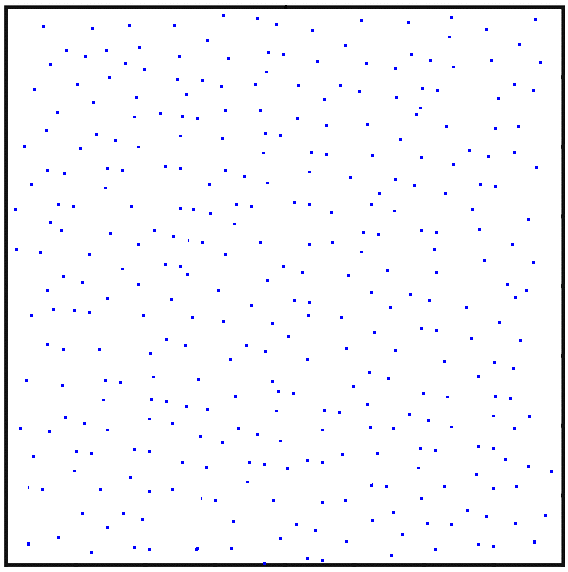
\includegraphics[scale=0.25]{./images/b0}
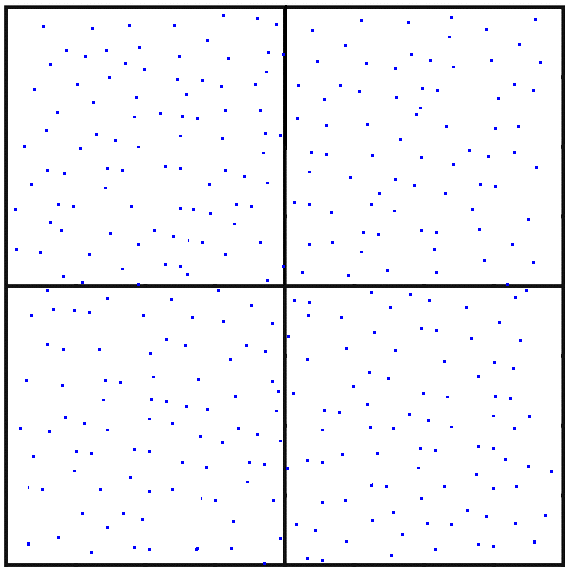
\includegraphics[scale=0.25]{./images/b1}
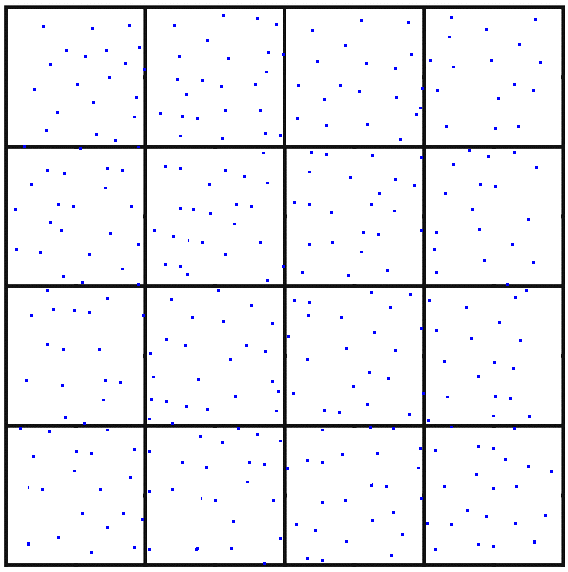
\includegraphics[scale=0.25]{./images/b2}
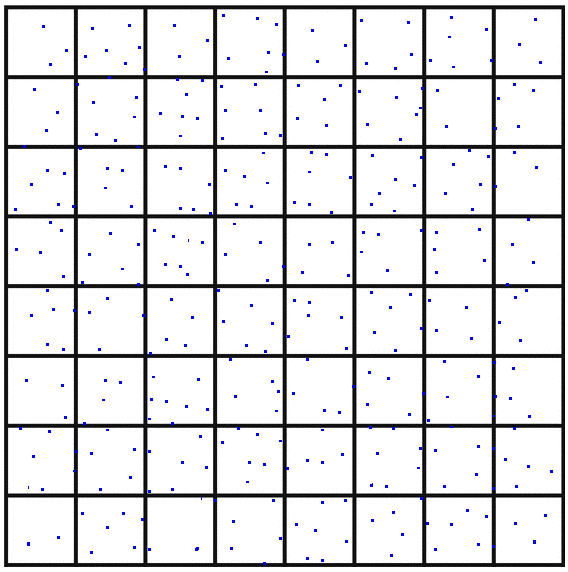
\includegraphics[scale=0.25]{./images/b3}
\end{figure}

We will use some terminology when discussing the tree, which we must define. A box's parent is the box one level up that contains it. Similarly a box's children are the boxes one level down that it contains. For example in Figure \ref{fig:4}, the only box on level $0$ is the parent of all boxes on level $1$. The near-neighbors of a box are the boxes on the same level with which it shares an edge or corner. In 2D, a box has at most $8$ near-neighbors. If two boxes are not near-neighbors they are called well-separated. A box's far-field is made up of all non-near-neighbor boxes. Lastly, each box has an interaction list, which is made up of boxes on the same level that are children of the parent's near-neighbors but are not near-neighbors. Figure \ref{fig:5} shows the interaction list of a box. Each box in 2D has at-most $27$, $6^2-3^2$, boxes in its interaction list.

\begin{figure}[h]
\caption{The blue boxes make up the interaction list of the red box.}
\label{fig:5}
\centering
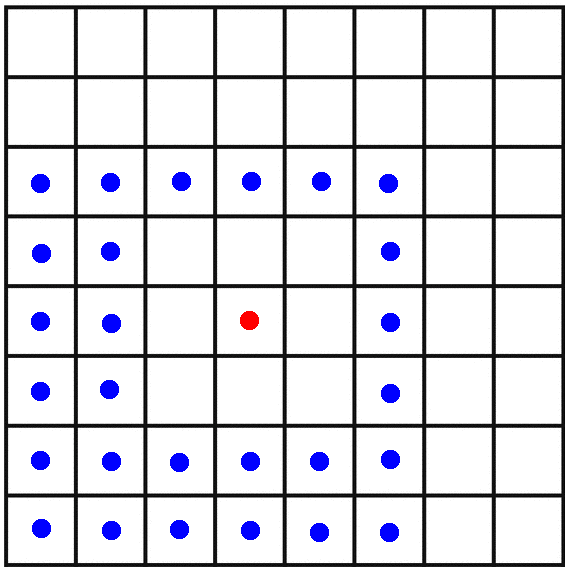
\includegraphics[scale=0.25]{./images/intlist}
\end{figure}

\subsection{Analysis-based FMMs}
The classical analysis-based FMM first developed by Greengard and Rokhlin in \cite{GR} relies on analytic expansions for the potential. As mentioned above, they used a multipole expansion such that sources clumped together could be viewed as a single source to a target in the far-field, and a local expansion to represent the potential at a target due to all sources in the far-field.

We now look at an example of these expansions. Consider the 2D single-layer Laplacian kernel $K(\mathbf{x},\mathbf{y})=-\frac{1}{2\pi}\log(|\mathbf{x}-\mathbf{y}|)$. It is convenient to write this as $K(\mathbf{x},\mathbf{y})=Re(\log(z_x-z_y))$, where $z_x$ and $z_y$ are complex number corresponding to points $\mathbf{x}$ and $\mathbf{y}$ in the plane. Now suppose the source densities are supported in a disk centered at $z_C$ with radius $r$. Then for all $z$ outside the disk with radius $R$, $(R > r)$, we can represent the potential at $z$ from the source densities using a set of coefficients $\{a_k ; 0 \le k \le p\}$, where
\begin{align}
f(z)=a_0\log(z-z_C)+\sum_{k=1}^p\frac{a_k}{(z-z_C)^k}+\mathcal{O}\bigg(\frac{r^p}{R^p}\bigg)
\end{align}
This is the multipole expansion. On the other hand, if the source densities are outside the disk with radius $R$, the potential at a point $z$ inside the disk with radius $r$ can be represented using a set of coefficients $\{c_k, 0\le k\le p\}$, where
\begin{align}
f(z)=\sum_{k=0}^pc_k(z-z_C)^k+\mathcal{O}\bigg(\frac{r^p}{R^p}\bigg)
\end{align}
This is the local expansion. In both expansions, $p$ is usually a small constant determined by the desired accuracy of the result. For 3D applications, rather than Laurent series', the far field is represented by expansions using spherical harmonics and Legendre polynomials.

For our problem of a modal FMM for axisymmetric density distributions, however, an analysis-based FMM for the series of modal Green's functions is not possible because the necessary analytic machinery (multipole and local expansions) for the modal Green's function, $s_n$, has not been found yet, if it exists at all. Even if it does exist, it is most likely inefficient to construct.

\subsection{Kernel-independent methods}
Since we don't have the analytic machinery required for an analysis-based FMM, we focus on kernel-independent methods to construct a modal FMM. One advantage of these methods is that they are relatively easy to implement, since in general they apply to an arbitrary kernel. To change the kernel in the classical FMM, we would need to develop analytic multipole and local expansions, which as aforementioned are difficult to find if they exist at all. These methods can be separated into two categories. The first requires that the kernel is the Green's function for some elliptic partial differential equation, satisfying Green's third identity. The most well-known method of this type is the kernel-independent FMM (KIFMM), which was constructed by Ying, Biros, and Zorin in \cite{YBZ}. Second are methods which work with any smooth kernel. The most well-known method of this type is the black-box FMM (bbFMM) by Fong and Darve in \cite{FD}.

Kernel-independent methods use equivalent densities to represent the source densities rather than analytic expansions. As an example, in the KIFMM, an upward equivalent density for a box is a continuous distribution surrounding the box that matches the potential due to the box's source densities at a target in the far-field. This is analogous to a multipole expansion. We find this density by solving the following equation for $\sigma^{B,u}$
\begin{align}
\int_{\mathbf{y}^{B,u}}{K(\mathbf{x},\mathbf{y})}\sigma^{B,u}{(\mathbf{y})}d\mathbf{y}=&\sum\limits_{j=1}^N K(\mathbf{x},\mathbf{y}_j)\sigma_j\mbox{ for all }\mathbf{x}\in\mathbf{x}^{B,u}
\end{align}
where $\mathbf{y}^{B,u}$ is the equivalent surface and $\mathbf{x}^{B,u}$ is the upward check surface, shown in Figure \ref{fig:6}. To solve, we discretize the equation using points on the equivalent and check surfaces, also shown in Figure \ref{fig:6}. This discretization requires two steps. First, the right hand side is the evaluation of a check potential. This step checks that the potential represented by the equivalent density and the actual source densities are the same to all boxes in the far field. Then on the left hand side, we invert a Dirichlet-type boundary integral equation to obtain the equivalent density. This corresponds to the application of a matrix of kernel evaluations. Similarly, the downward equivalent density for a box is a continuous distribution surrounding the box that matches the potential at a target in the box due to all source densities in the far field. To get this, again we solve a boundary integral equation using a discretization scheme. This is analogous to the local expansion in the analysis-based FMM. Using these densities, the KIFMM only requires kernel evaluations.

\begin{figure}[h]
\caption{The red circle is the upward equivalent surface with dark red discretization points. The blue circle is the upward check surface with light blue discretization points.}
\label{fig:6}
\centering
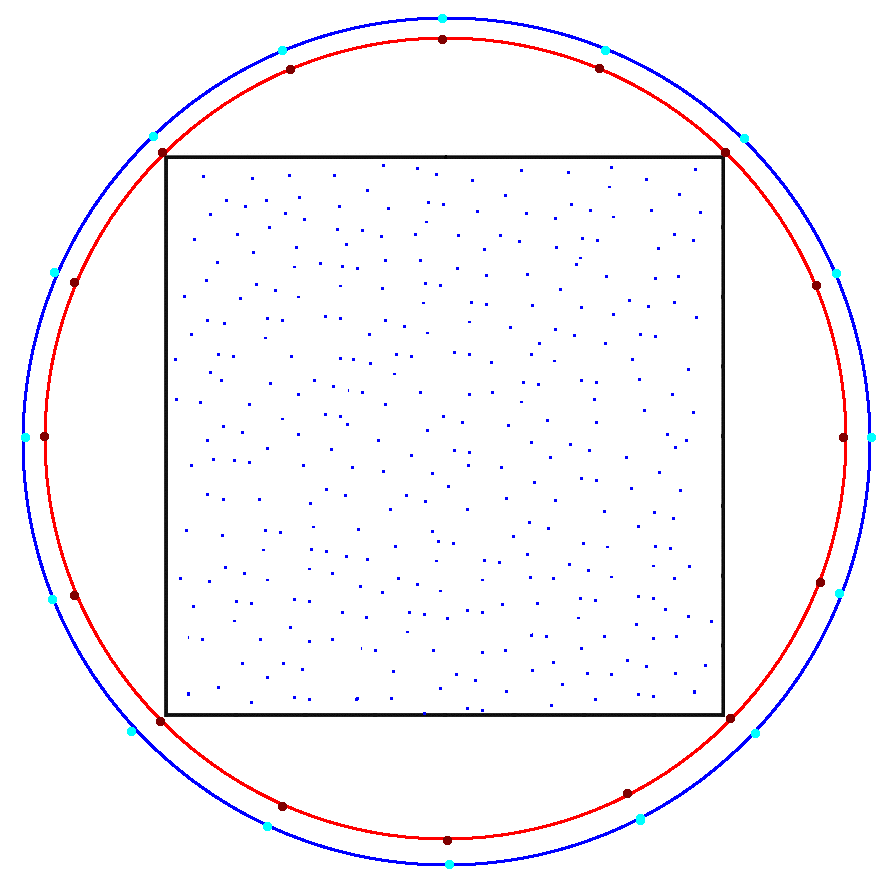
\includegraphics[scale=0.25]{./images/eqdens1}
\end{figure}

Before we address the application of the KIFMM to an axisymmetric density distribution, we discuss translation operators and the general structure of the FMMs. These two elements need to be covered to understand the inefficiencies of the KIFMM as a basis for the modal FMM in this scenario.

\subsection{Translation operators}
FMMs employ these multipole and local expansions or upward and downward equivalent densities recursively in a multilevel scheme. Translations between these efficient representations are what make these $\mathcal{O}(N)$ algorithms possible.

In the analysis-based FMM, a translation operator translates a multipole or local expansion of one box to that of another in the computational domain using expansions of functions. In kernel-independent methods, translation operators translate equivalent densities in the same way but with linear operators or matrices. To describe each operator below, we use the terminology for the analysis-based FMM (multipole and local expansions), but we could analogously substitute upward and downward equivalent densities. In particular, five translations are used:

\begin{itemize}
\item $S2M$: The source to multipole operator creates a multipole expansion for a box.

\item $M2M$: The multipole to multipole operator translates the multipole expansion of a box to that of its parent.

\item $M2L$: The multipole to local operator translates the multipole expansion of a box to the local expansion of a box in its interaction list.

\item $L2L$: The local to local operator translates the local expansion of a box to the local expansion of a child box.

\item $L2T$: The local to target operator computes the far-field interaction contribution by evaluating the local expansion of a box at the target points in that box.
\end{itemize}

It's important to note that the sum of the contributions from the $M2L$ operation and $L2L$ operation make up the local expansion, or downward equivalent density, for a box.

These translation operators are the backbone of a fast multipole algorithm because they reduce the number of direct computations required to do the summation in equation $(1)$. The $M2M$, $M2L$, and $L2L$ translation operators can be computed without any knowledge of the source or target points, so they are a true pre-computation. The only requirement is a partitioned computational domain.

An important consideration in evaluating a fast method is the cost of pre-computing these operators. For translation invariant kernels, the translation operators will only differ based on relative position and level in the hierarchical tree. This is due to the fact that the kernel only depends on the difference between coordinate values, $(|\mathbf{x}-\mathbf{y}|)$. For example, using Figure \ref{fig:7}, with a translation invariant kernel the $M2L$ operator used to translate from the green box to the orange box would be the same one used to translate from the blue box to the red box. So in the case of translation invariant kernels, many $M2L$ translation operators on a given level are identical, and need not be computed repeatedly. In fact, each level has at most $40$ $(7^2-3^2)$ unique transfer vectors in this case.

\begin{figure}[h]
\caption{We use this figure to describe relationships between translation operators.}
\label{fig:7}
\centering
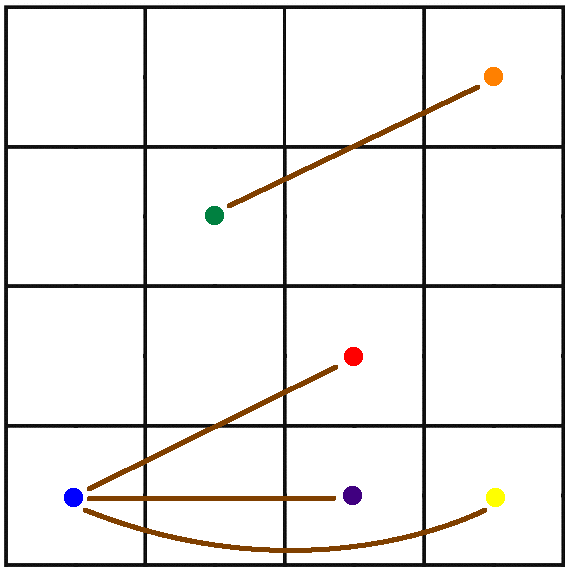
\includegraphics[scale=0.25]{./images/M2L}
\end{figure}

On the other hand, for kernels that are not translation invariant in any variable, every translation operator for every box in the computational domain needs to be computed. Every transfer vector is unique, so none of them can be reused or recycled as above. Notice that the modal Green's function is invariant in $z$, but not $r$, so we need to take this more costly pre-computation into consideration. In particular, this is a negative aspect of using the KIFMM for axisymmetric densities, which we discuss in $\S4.6$.

\subsection{General multilevel algorithm}
Now that we've defined the tree structure and translation operators, we can give the general algorithmic structure for FMMs. All of these methods, whether analysis-based or kernel-independent, use the same general steps to accelerate the summation in equation $(1)$. This is shown in \cite{FD}, \cite{GR}, \cite{YBZ}, and many other FMM papers. Here we'll continue to work in 2D, and use terminology from kernel-independent methods (upward and downward equivalent densities), although we could analogously substitute the analysis-based FMM language.
\begin{enumerate}
\item Hierarchically partition the computational domain using a quadtree of boxes with $L+1$ levels $0,\dots,L$, until each box on the finest level $L$ contains no more than $p$ source points. The parameter $p$ is chosen based on a desired accuracy level $\epsilon$.
\item For each box on the finest level $L$, construct an upward equivalent density using the $S2M$ operator.
\item For each box on levels $1,\dots,L$, shift the upward equivalent density of the box to the upward equivalent density of the parent box using the $M2M$ operator. Steps $3$ and $4$ are referred to as the upward pass, and together they accumulate upward equivalent densities for every box in the computational domain.
\item For each box on levels $2,\dots,L$, compute the contribution to the box's downward equivalent density by translating the upward equivalent densities of boxes in its interaction list using the $M2L$ operator.
\item For each box on levels $0,\dots,L-1$, translate the downward equivalent density of the box to the downward equivalent densities of its child boxes using the $L2L$ operator. Steps $4$ and $5$ are referred to as the downward pass, and the summation of these operations accumulates a downward equivalent density for every box in the computational domain.
\item Compute the total far-field contribution for each box by using the $L2T$ operator to evaluate its downward equivalent density at the target points in the box.
\item Lastly, for each box, directly compute the contribution from near-field interactions from sources in near-neighbor boxes and add them to the far-field contribution. This sum is the total potential at targets in the box.
\end{enumerate}

\subsection{Problems with a modal KIFMM}
As explained in $\S4.3$, rather than using analytic multipole and local expansions, the KIFMM substitutes a continuous distribution of upward and downward equivalent densities that lie on surfaces surrounding each box in the hierarchical tree to represent the potential generated by sources in that box and the potential in that box due to sources in the far-field.

To implement the KIFMM for axisymmetric density distributions, the technique of using the modal Green's functions described at length by Young, Yao, and Martinsson in \cite{YYM} can be used; replace the 3D integral equations required by the 3D KIFMM with their Fourier representations, sequences of 2D integral equations. This way we can avoid the 3D KIFMM in favor of repeatedly applying the 2D KIFMM.

There are, however, a few negative attributes of using the KIFMM as the basis for a modal FMM. The first is that the pre-computation of translation operators will be expensive due to the fact that the modal Green's function is not a translation invariant kernel. As aforementioned, for non-translation invariant kernels, we need to pre-compute all translation operators for every box in the computational domain. In an attempt to reduce this pre-computation, we tried to find constant proportionality between the operators. For example, using Figure \ref{fig:7} we considered that perhaps the $M2L$ operator used to translate from the blue box to the purple box is in proportion to the $M2L$ operator used to translate from the blue box to the yellow box. However, these attempts failed and indeed since the translation operators in the KIFMM are simply kernel evaluations, we wouldn't expect to find this proportionality in them because it doesn't exist in the kernel. So every translation operator for every box on every level would need to be pre-computed.

Further adding to the pre-computation is the fact that these operators need to be computed for all $2M+1$ modes, where $M$ is the truncation parameter for the Fourier expansion. As we saw in $\S4.5$, the translation operators in the KIFMM in their discretized form are matrices of kernel evaluations that translate an equivalent density from one box to that of another. Since we're essentially using $2M+1$ different kernels in this scenario, then the algorithm will require the pre-computation of $2M+1$ times the number of operators required for the computational domain. The consequences of translation operators made up of kernel evaluations is not limited to the pre-computation. The result is essentially that the entire FMM algorithm described in $\S4.5$ would need to be done separately $2M+1$ times, once for each mode of the kernel. This is in sharp contrast to the computational savings of the vectorization of this process that's possible in the black-box FMM, which we discuss next.

\section{The black-box FMM}
The black-box FMM is a kernel-independent, Chebyshev interpolation-based $\mathcal{O}(N)$ algorithm for non-oscillatory kernels. Over the course of this section, we will show that the bbFMM will serve as a strong basis for developing a modal FMM. In particular, we consider this scheme to quickly compute this sum for each modal Green's function
\begin{align}
f_m(\mathbf{x}_i)=\sum_{j=1}^N s_m(\mathbf{x}_i,\mathbf{y}_j)\sigma_{m,j}
\end{align}
for targets $\mathbf{x}_i$ and sources $\mathbf{y}_j$.

The full fast summation algorithm combines the methods of SVD compression from \cite{ZGR} and \cite{MR}, which gives the kernel approximation
\begin{align}
s_m(\mathbf{x},\mathbf{y})=\sum_i \alpha_i u_i(\mathbf{x})v_i(\mathbf{y})
\end{align}
and Chebyshev interpolation, which gives the kernel approximation
\begin{align}
s_m(\mathbf{x},\mathbf{y})=\sum_i\sum_j s_m(\mathbf{x}_i,\mathbf{y}_j)w_i(\mathbf{x})w_j(\mathbf{y})
\end{align}

The advantages of this method for axisymmetric density distributions with difficult geometries are many. In general, this algorithm uses weights in each box placed at Chebyshev nodes as equivalent densities. As a consequence of discretizing an integral equation of the type in equation $(1)$, we need a numerical quadrature rule that has more discretization points in corners or near geometric singularities. Chebyshev nodes clump in corners such that source densities located there will be well-represented. The location of these weights is shown in Figure \ref{fig:8}. The bbFMM is also good for analytically complicated kernels like the modal Green's function, $s_m$, but which can be evaluated efficiently as shown in \cite{HK} and \cite{YYM}. Unlike the FMM or KIFMM, the bbFMM just requires a smooth kernel, and only uses kernel evaluations at Chebyshev nodes.

\begin{figure}[h]
\caption{The bbFMM uses equivalent densities in the form of weights at the Chebyshev nodes in each box to represent the source densities. This is shown for $n^2=100$ Chebyshev nodes in red representing the source densities in blue.}
\label{fig:8}
\centering
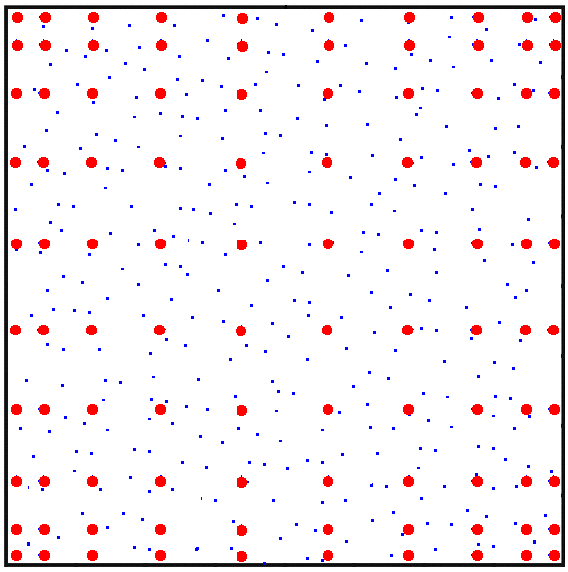
\includegraphics[scale=0.25]{./images/b0wChebynodes}
\end{figure}

To take a step back and find these Chebyshev nodes, we need to define the $n$th Chebyshev polynomial
\begin{align*}
T_n(x)=\cos\bigg(n\arccos\bigg(\frac{2}{b-a}\bigg(x-\frac{a+b}{2}\bigg)\bigg)\bigg)
\end{align*}
on an interval $[a,b]$. In one dimension, the Chebyshev nodes are the $n$ roots of the Chebyshev polynomial on $[a,b]$
\begin{align*}
\mathbf{\overline{x}}_i=\frac{a+b}{2}+\frac{b-a}{2}\cos\bigg(\frac{2i-1}{2n}\pi\bigg)\mbox{ for }i=1,\dots,n.
\end{align*}
For two dimensions, there are $n^2$ Chebyshev nodes that are the tensor product of the Chebyshev nodes of each interval on the $r$ and $z$ axes.

From the Chebyshev polynomials Fong and Darve derive the interpolation functions
\begin{align*}
R_n(\mathbf{x},\mathbf{y}) = \bigg(\frac{1}{n} + \frac{2}{n}\sum_{i=1}^{n-1}T_n(r)T_n(z)\bigg)\bigg(\frac{1}{n} + \frac{2}{n}\sum_{i=1}^{n-1}T_n(r')T_n(z')\bigg)
\end{align*}
for $\mathbf{x}=(r,z)$ and $\mathbf{y}=(r',z')$. From there we can construct a low-rank approximation for the $m$th modal Green's function given by
\begin{align}
s_m(\mathbf{x},\mathbf{y}) = \sum_{l_1=1}^n\sum_{l_2=1}^n\sum_{m_1=1}^n\sum_{m_2=1}^n s_m(\mathbf{\overline{x}}_{l_1,l_2},\mathbf{\overline{y}}_{m_1,m_2})R_n(\mathbf{\overline{x}}_{l_1,l_2},\mathbf{x})R_n(\mathbf{\overline{y}}_{m_1,m_2},\mathbf{y})
\end{align}
and apply it to approximate the sum in equation $(12)$ by
\begin{align}
f_m(\mathbf{x}_i)=\sum_{l_1=1}^n \sum_{l_2=1}^n R_n(\mathbf{\overline{x}}_{l_1,l_2},\mathbf{x}_i) \sum_{m_1=1}^n \sum_{m_2=1}^n s_m(\mathbf{\overline{x}}_{l_1,l_2},\mathbf{\overline{y}}_{m_1,m_2}) \sum_{j=1}^N \sigma_{m,j}R_n(\mathbf{\overline{y}}_{m_1,m_2},\mathbf{y}_j)
\end{align}
where $\mathbf{\overline{x}}_{l_1,l_2}$ are the Chebyshev nodes in the target box, and $\mathbf{\overline{y}}_{m_1,m_2}$ are the Chebyshev nodes in the source box.

\subsection{Translation operators}
This low-rank approximation in equation $(18)$ yields translation operators for this method. For a given mode $m$, we detail each operation.
\begin{itemize}
\item $S2M$: The source-to-multipole operation computes weights $W^{m,B}_{m_1,m_2}$ at each Chebyshev node $\mathbf{\overline{y}}_{m_1,m_2}$ by anterpolation in a box $B$.
\begin{align}
W_{m_1,m_2}^{m,B} = \sum_{\mathbf{y}_j\in B} \sigma_{m,j} R_n(\mathbf{\overline{y}}^B_{m_1,m_2},\mathbf{\overline{y}}_j)
\end{align}
for $m_i = 1,\dots,n$.
\item $M2M$: The multipole-to-multipole operation translates weights at the nodes of four child boxes $B_i$, $W_{m_1,m_2}^{m,B_i}$, to weights at the nodes of its parent box $A$, $W_{m_1,m_2}^{m,A}$.
\begin{align}
W_{m_1,m_2}^{m,A} = \sum_{i=1}^4 \sum_{m'_1=1}^n\sum_{m'_2=1}^n W_{m'_1,m'_2}^{m,B_i} R_n(\mathbf{\overline{y}}^A_{m_1,m_2},\mathbf{\overline{y}}^{B_i}_{m'_1,m'_2})
\end{align}
for $m_i= 1,\dots,n$.
\item $M2L$: The multipole-to-local operation computes the far-field contribution at Chebyshev nodes $\mathbf{\overline{x}}_{l_1,l_2}^A$ in box $A$ from all boxes $B_i$ in the interaction list of $A$.
\begin{align}
g_{l_1,l_2}^{m,A} = \sum_{B_i} \sum_{m_1=1}^n\sum_{m_2=1}^n W_{m_1,m_2}^{m,B_i} s_m(\mathbf{\overline{x}}^{A}_{l_1,l_2},\mathbf{\overline{y}}^{B_i}_{m_1,m_2})
\end{align}
for $l_i = 1,\dots,n$.
\item $L2L$: On the root level let $f^{m,A}_{l_1,l_2}=g^{m,A}_{l_1,l_2}$ and use the local-to-local operation to obtain the full local expansion by adding the far-field contribution from the parent box $B$
\begin{align}
f^{m,A}_{l_1,l_2}=g^{m,A}_{l_1,l_2} + \sum_{l'_1=1}^n \sum_{l'_2=1}^n f^{m,B}_{l_1,l_2} R_n(\mathbf{\overline{x}}_{l_1,l_2}^A,\mathbf{\overline{x}}_{l'_1,l'_2}^B)
\end{align}
for $l_i = 1,\dots,n$ where $B$ is the parent box of box $A$. This $f$ is analogous to the local expansion in the analysis-based FMM.
\item $L2T$: The local-to-target operation computes $f_m(\mathbf{x}_i)$ for target point $\mathbf{x}_i$ in box $B$ by interpolating the far-field approximation.
\begin{align}
f_m(\mathbf{x}_i)=\sum_{l_1=1}^n \sum_{l_2=1}^n f^{m,B}_{l_1,l_2} R_n(\mathbf{\overline{x}}_{l_1,l_2}^B,\mathbf{x}_i)
\end{align}
\end{itemize}
In general, one advantage of the bbFMM is a small pre-computation even for large systems. The pre-computation for any kernel (even not translation invariant) is just $\mathcal{O}(N)$. This is due to the fact that we don't need kernel evaluations, which are costly, to obtain all but the $M2L$ operators. In the case of the modal Green's function, we have another pre-computational advantage. Since the $S2M$, $M2M$, $L2L$, and $L2T$, translation operators in this scenario only depend on the interpolation functions $R_n$, then they are constant over all $2M+1$ modes. So we only need to be pre-compute one set of these operators, instead of $2M+1$ separate sets (one for each mode) as in the KIFMM.

\subsection{Vectorization of the bbFMM for the modal Green's function}
A huge disadvantage of the KIFMM was that we would need to separately complete the entire algorithm $2M+1$ times to account for each node. In contrast, with the bbFMM, we can utilize a matrix representation that includes all Chebyshev nodes and all Fourier modes to further accelerate translation operations. We call this representation the vectorization of the bbFMM for the modal Green's function.

Consider $\sigma_m,j$ is the charge of  the $j$th source in the $m$th Fourier mode of $\sigma$ as in $\S3.1$. We can represent this as the $m,j$th entry in a $(2M+1)\times N$ matrix. Performing the $S2M$ step for all modes is now a matrix-matrix multiplication with the analogously-defined $N\times n^2$ matrix with interpolation function entries $R_n(\mathbf{\overline{y}}_{m_1,m_2},\mathbf{y}_j)$. The result is the equivalent density matrix $[W^{m,B}_{m_1,m_2}]$, which has $2M+1$ rows (one for each Fourier mode), and $n^2$ columns (one for each Chebyshev node).

Further translation operations can now be computed as using matrix operations as well, which in practice can be performed quickly. Using this vectorization representation, we can perform the $S2M$, $M2M$, $L2L$, and $L2T$ operations for every mode at once, rather than $2M+1$ separate runs as in the KIFMM, which is a big computational advantage.

\subsection{Accelerating the $M2L$ operation}
The $M2L$ operation deserves special attention because it does depend on the kernel $s_m$ and is the most expensive operator to pre-compute and to apply as well. That being said, there are many techniques for accelerating not only the pre-computation of the $M2L$ operator but also its application as described in \cite{A}, \cite{CGMR}, \cite{FD}, \cite{MR}, and \cite{VBT}.

The computation of the $s_m$, not to be confused with its evaluation, using the Fast Fourier Transform (FFT), generates each of the $2M+1$ Fourier modes all at once. We know that $s_m$ satisfies the following equation as stated in $\S3.1$,
\begin{align}
s_m = \int_0^{2\pi} \frac{1}{4\pi|\mathbf{x}-\mathbf{y}|}e^{-im\theta'}d\theta'
\end{align}
So for $x$ and $y$ well-separated, we can use the discrete FFT on $|x-y|$ to get all modes $s_m$ for use in the M2L.

Once we have the modal Green's functions $s_m$, they can be evaluated efficiently using techniques described in \cite{A}, \cite{VBT}, and others. The full bbFMM in \cite{FD} also includes a reduction of the cost of the $M2L$ operation by using SVD compression, based on results in \cite{CGMR} and \cite{MR}.

\section{Conclusion and Future Work}
We need to complete the full algorithm for the modal FMM based on the bbFMM, fully utilizing the efficient pre-computation, vectorization, and $M2L$ acceleration. Once this is complete, we can test the full implementation.

\begin{appendices}
\section{Legend}
\begin{align*}
&N \mbox{ the number of source points in the computational domain}\\
&m \mbox{ the index for each Fourier mode of the Green's function}\\
&M \mbox{ the truncation parameter for the Fourier expansion of the Green's function}\\
&n \mbox{ the number of Chebyshev nodes in each interval}\\
&\mathbf{x}_i\mbox{ target points}\\
&\mathbf{\overline{x}}_{l_1,l_2}\mbox{ Chebyshev nodes in the target box}\\
&\mathbf{y}_j\mbox{ source points}\\
&\mathbf{\overline{y}}_{m_1,m_2}\mbox{ Chebyshev nodes in the source box}\\
\end{align*}

\section{Implementation and Testing}
Currently, we are able to produce and have tested all equivalent densities and translation operators with Python programs for the Chebyshev interpolation-based bbFMM. However, for now we are just using the kernel, $\log|\mathbf{x}-\mathbf{y}|$, for ease of evaluation, instead of the modal Green's function for Laplace's equation. However, these functions are very similar so we expect these tests to succeed with the modal Green's function as well.

Much of the future work to do is a full FMM implementation in Python. Key pieces of this will be accelerating the $M2L$ operation by efficiently evaluating the modal Green's function, using the vectorization discussed in $\S6$, and using singular value decomposition (SVD) compression technique described in \cite{CGMR}, \cite{FD}, \cite{ZGR} and \cite{MV}.

The following are descriptions of the computations done by each of our test programs. These tests are standard practice to debug translation operators.
\begin{itemize}
\item $\mathbf{S2M.py}$
\begin{enumerate}
\item Put $N$ sources in box $A$ and assign charges of $\pm 1$.
\item Put target in a box $B$ in the far field.
\item For each Chebyshev node of $A$, assign a weight\\
$$W_{m_1,m_2}=\sum_{j=1}^N \sigma_j R_n(\mathbf{\overline{y}}_{m_1,m_2},\mathbf{y}_j)$$
\item Compute the potential at each Chebyshev node in a target box $B$\\
$$f_{l_1,l_2}=\sum_{m_1=1}^n\sum_{m_2=1}^n W_{m_1,m_2} \log(\mathbf{\overline{x}}_{l_1,l_2},\mathbf{\overline{y}}_{m_1,m_2})$$
\item Compute the potential at the target by interpolation\\
$$f(\mathbf{x}_i)=\sum_{l_1=1}^n\sum_{l_2=1}^n f_{l_1,l_2} R_n(\mathbf{\overline{x}}_{l_1,l_2},\mathbf{x}_i)$$
\item Compare the result with the naive computation of the potential\\
$$f(\mathbf{x}_i)=\sum_{j=1}^N \log(\mathbf{x}_i,\mathbf{y}_j) \sigma_j$$
\end{enumerate}

\item $\mathbf{M2M}$
\begin{enumerate}
\item Put $N$ sources in box $A$ and assign charges of $\pm 1$.
\item For each Chebyshev node of $A$, assign a weight\\
$$W_{m_1,m_2}=\sum_{j=1}^N \sigma_jR_k(\mathbf{\overline{y}}_{m_1,m_2},\mathbf{y}_j)$$
\item Repeat step $2$ for the four child boxes $B_i$ of $A$. Note that there will be $\le N$ sources in each child box.
\item Use the $M2M$ operation to compute\\
$$W^A_{m_1,m_2}= \sum_{i=1}^4\sum_{m'_1=1}^n\sum_{m'_2=1}^n R_n(\mathbf{\overline{x}}^{A}_{m_1,m_2},\mathbf{\overline{x}}^{B_i}_{m'_1,m'_2})W^{B_i}_{m'_1,m'_2}$$
\item Compare the weight at each node with the computation in step $2$.
\end{enumerate}
Note that at this point if the weights match, there is no need to make sure the potential estimates match the naive potential computation.\\

\item $\mathbf{M2L.py}$\\
Note that this is the case where there is no $L2L$ contribution to the local expansion of a box $B$, since the parent of $B$ has no interaction list.
\begin{enumerate}
\item Put a target point in a box $B$.
\item Put $N$ sources in each box $I_i$ in the interaction list of $B$ and assign charges of $\pm 1$.
\item For each Chebyshev node of $I_i$, assign a weight
$$W^{I_i}_{m_1,m_2}=\sum_{j=1}^N \sigma^{I_i}_j R_n(\mathbf{\overline{y}}_{m_1,m_2},\mathbf{y}^{I_i}_j)$$
\item Calculate the far-field contribution at the Chebyshev nodes of $B$
$$f_{l_1,l_2}=\sum_{I_i}\sum_{m_1=1}^n\sum_{m_2=1}^n W^{I_i}_{m_1,m_2} \log(\mathbf{\overline{x}}^{B}_{l_1,l_2},\mathbf{\overline{y}}^{I_i}_{m_1,m_2})$$
\item Compute the potential at the target point by interpolation
$$f(\mathbf{x}_i)=\sum_{l_1=1}^n\sum_{l_2=1}^n f_{l_1,l_2} R_n(\mathbf{\overline{x}}_{l_1,l_2},\mathbf{x}_i)$$
\item Compare the result with the naive computation of the potential\\
$$f(\mathbf{x}_i)=\sum_{I_i}\sum_{j=1}^N \log(\mathbf{x}_i,\mathbf{y}^{I_i}_j) \sigma^{I_i}_j$$
\end{enumerate}

\item $\mathbf{L2L.py}$\\
Note that this is the case where there is no $M2L$ contribution to the local expansion of a target box $B$, since $B$ has no interaction list. 
\begin{enumerate}
\item Put a target point in a box $B$, with parent box $P$.
\item Put $N$ sources in each box $I_i$ in the interaction list of $P$ and assign charges of $\pm 1$.
\item For each Chebyshev node of $I_i$, assign a weight
$$W^{I_i}_{m_1,m_2}=\sum_{j=1}^N \sigma^{I_i}_j R_n(\mathbf{\overline{y}}_{m_1,m_2},\mathbf{y}^{I_i}_j)$$
\item Calculate the far-field contribution at the Chebyshev nodes of the parent of $B$
$$f_{l_1,l_2}=\sum_{I_i}\sum_{m_1=1}^n\sum_{m_2=1}^n W^{I_i}_{m_1,m_2} \log(\mathbf{\overline{x}}^{P}_{l_1,l_2},\mathbf{\overline{y}}^{I_i}_{m_1,m_2})$$
\item Compute the potential at the target point by interpolation
$$f(\mathbf{x}_i)=\sum_{l_1=1}^n\sum_{l_2=1}^n f_{l_1,l_2} R_n(\mathbf{\overline{x}}_{l_1,l_2},\mathbf{x}_i)$$
\item Compare the result with the naive computation of the potential\\
$$f(\mathbf{x}_i)=\sum_{I_i}\sum_{j=1}^N \log(\mathbf{x}_i,\mathbf{y}^{I_i}_j) \sigma^{I_i}_j$$
\end{enumerate}
\end{itemize}
Note that in the case where there is a contribution from both the $M2L$ and $L2L$ operations, the local expansion is simply the sum of these contributions. Also note that the efficacy of the $L2T$ computation is shown in the last step of the $S2M$, $M2L$, and $L2L$ computations.
\end{appendices}

\begin{thebibliography}{99}\addcontentsline{toc}{chapter}{Bibliography}

\bibitem{A} Adbelmageed, A., \emph{Efficient Evaluation of Modal Green's Functions Arising in EM Scattering by Bodies of Revolution}. Progress in Electromagnetics Research, PIER 27, (2000), 337-356.

\bibitem{CGMR} Cheng, H., Gimbutas, Z., Martinsson, P.G., Rokhlin, V., \emph{On the Compression of Low Rank Matrices}. SIAM Journal of Scientific Computing, 26(4), (2005), 1389-1404.

\bibitem{FD} Fong, W., Darve, E., \emph{A black-box fast multipole method}. Journal of Computational Physics, 228, (2009), 8712-8725.

\bibitem{ZGR} Gimbutas, Z., Rokhlin, V., \emph{A Generalized Fast Multipole Method for Nonoscillatory Kernels}. SIAM Journal of Scientific Computing, 24(3), (2002), 796-817.

\bibitem{GR} Greengard, L., Rokhlin, V., \emph{A Fast Algorithm for Particle Simulations}. Journal of Computational Physics, 73, (1987), 325-348.

\bibitem{HMY} Hao, S., Martinsson, P.G., Young, P., \emph{An efficient and highly accurate solver for multi-body acoustic scattering problems involving rotationally symmetric scatterers}. Computers and Mathematics with Applications, 69, (2015), 304-318.

\bibitem{HK} Helsing, J., Karlsson, A., \emph{An explicit kernel-split panel-based Nystr{\"o}m scheme for integral equations on axially symmetric surfaces}, \textbf{arxiv.org/abs/1310.4715}, (2014).

\bibitem{MR} Martinsson, P.G., Rokhlin, V., \emph{An accelerated kernel-independent fast multipole method in one dimension}. SIAM Journal of Scientific Computing, Vol. 29, No. 3, (2007), 1160-1178.

\bibitem{VBT} Vaessen, J.A.H.M., van Beurden, M.C., Tijhuis, A.G., \emph{Accurate and Efficient Computation of the Modal Green's Function Arising in the Electric Field Integral Equation for a Body of Revolution}. IEEE Transactions on Antennas and Propagation, 60(7), (2012), 3294-3304.

\bibitem{YBZ} Ying, L., Biros, G., Zorin, D., \emph{A kernel-independent adaptive fast multipole method algorithm in two and three dimensions}. Journal of Computational Physics, 196, (2004), 591-626.

\bibitem{YYM} Young, P., Yao, S., Martinsson, P.G., \emph{A high-order Nystr{\"o}m discretization scheme for boundary integral equations defined on rotationally symmetric surfaces}. Journal of Computational Physics, 231, (2012), 4142-4159.

\end{thebibliography}
\end{document}



